\chapter{Methodology}
\label{ch:methodology}

This chapter delves into the methodology employed to address the research questions and objectives outlined in the previous chapters.
The chapter is organized into three main sections.
\autoref{ch:architecture} discusses the architecture of our proposed solution, elaborating on the tabular processor and its implementations, namely the BGMProcessor and FTProcessor.
In addition, this section also highlights the modifications made to the existing software to incorporate the proposed solutions.

\autoref{ch:methods-experimentalSetup} focuses on the experimental setup, outlining the experiments conducted to evaluate the performance and effectiveness of the proposed models.
It provides detailed information on the execution environment and the hyperparameter search space used in the study, ensuring the reproducibility of the results.

Finally, \autoref{ch:methods-datasets} presents the dataset utilized in the experiments, including its source and characteristics.
This information is crucial to understanding the context in which our proposed methodology was tested and evaluated.

By the end of this chapter, the reader will gain a comprehensive understanding of the methodology implemented in this thesis, which will lead to the presentation and analysis of the results in the subsequent chapters.

\section{Architecture}
\label{ch:architecture}

The software's architecture was developed with the requirements in \autoref{ch:requirements} in mind.
The following section will explain how the individual additions to the existing code are designed and why the design was chosen.


\subsection{Tabular Processor}
\label{ch:architecture-tabularProcessor}

To allow for flexible use and the possibility of adding additional processing mechanisms (R5 - Maintainability), the \textit{strategy design} pattern (\autoref{fig:design}) was chosen \cite{gamma1994design}.
The pattern is beneficial if a specific behavior is required, but needs to be realized in different ways.
The \textit{Strategy} class defines what kind of methods need to be implemented and what behavior the class should have.
The \textit{Strategy} classes children define a \textit{ConcreteStrategy} and realize the desired behavior in different ways.
Different \textit{ConcreteStrategies} can be used interchangeably independent of the \textit{Context} they are used in since all implement the same functionalities.
The \textit{Context} is has a reference to the \textit{ConcreteStrategies} and ultimately decides when an instance of type \textit{Strategy} is executed.
As the \textit{ConcreteStrategies} implement the same interface, the \textit{Context} can execute any function a \textit{ConcreteStrategies} has implemented, without needing to know the inner workings of that function.
Hence, whenever the \textit{Context} needs to execute a certain functionality, it delegates the execution to the \textit{ConcreteStrategy} object it needs, which may vary on the situation.
One of the biggest advantages is, that this way new \textit{ConcreteStrategies} can be added easily without affecting any of the other \textit{ConcreteStrategy} or the \textit{Context} \cite{gamma1994design}.

\begin{figure}[h]
	\centering
	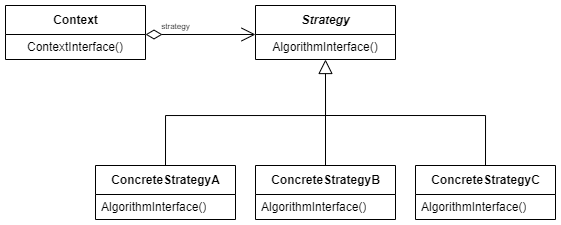
\includegraphics[width=0.8\textwidth]{images/strategy.png}
	\caption[Strategy Design Pattern]{Strategy design pattern \cite[p. 316]{gamma1994design}}
	\label{fig:design}
\end{figure}

\begin{figure}[h]
	\centering
	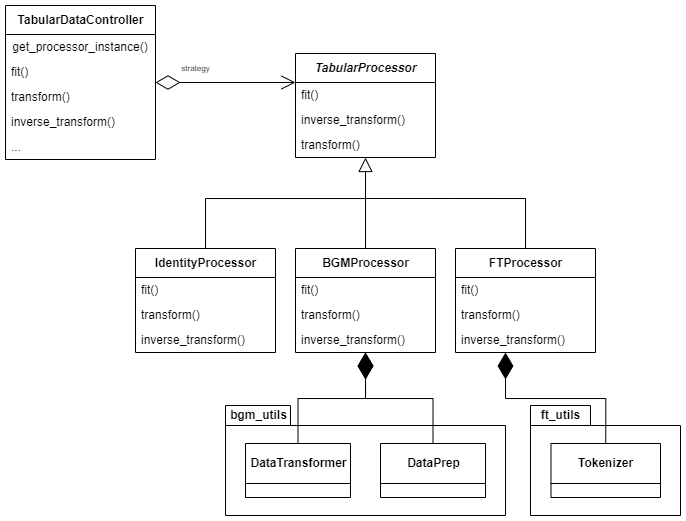
\includegraphics[width=0.8\textwidth]{images/tabular_processor.png}
	\caption[Tabular Processor Design]{Tabular Processor Design}
	\label{fig:tabular_processor}
\end{figure}

\autoref{fig:tabular_processor} shows how the \textit{strategy design} pattern is realized.
The overall \textit{Strategy} class is defined in the \textit{TabularProcessor} class in the form of an abstract class with three core methods each tabular processing mechanism needs to implement.
These functions are the \textit{fit}, \textit{transform}, and \textit{inverse transform} functions (FR2.1 - FR2.3).

Each tabular processing strategy is different and realizes the transformation of the data in a different way by implementing the abstract functions of the parent strategy.
Therefore, new tabular processing mechanisms can be easily added by just implementing the methods of the abstract class (R2, FR2).
Furthermore, the tabular processing mechanism can be exchanged easily since they share the same functions.
This is handled in the \textit{TabularDataController} class, which is equivalent to the \textit{Context} of the \textit{strategy design} pattern.
The \textit{TabularDataController} handles all relevant aspects to use the tabular processing mechanisms, including but not limited to the instantiation, fitting, saving, and loading of \textit{TabularProcessor} instances.
The data, whose columns are segmented into categorical, numerical, and target as numpy arrays \cite{harris2020array}, needs to be provided to instantiate a tabular processor.
Target refers to the column of the dataset that a model tries to predict or estimate in a classification or regression scenario.
The first step in using the tabular processor is fitting it to the data.
Additional information required for the fitting process can be provided through meta-data in the form of a dictionary, which may change for different realizations.
Note that this fit function might not be necessary, depending on the processing mechanism, but it is required to be implemented anyways.
Only after fitting the transform function can be called transforming the data format and returning the transformed data in the same data segmentation structure, \ie separated into categorical, numerical and target arrays.
The inverse transformation works similarly, reversing transformed data back to its original format.
For clarity, please note the difference between the terms "data format" and "data segmentation" in this thesis.
The term "data segmentation" refers to the separation of columns into categorical, numerical, and target segments.
On the other hand, the term "data format" refers to the modification of the data values achieved through the encoding and decoding processes of the \textit{TabularProcessor}, specifically via their "transform" and "inverse transform" functions.

\subsection{Tabular Processor Implementations}
\label{ch:architecture-tabularProcessor-implementations}

Three different tabular processor versions have been implemented.
The \textit{IdentityProcessor} does not do anything to the data.
It is used to do experiments without any tabular processing mechanism and allows reproducing the original results of \cite{kotelnikov2022TabDDPMModellingTabular}.
In this thesis, only two approaches have been implemented, the \gls{bgm} and \gls{ft} tabular processors.
Other potential tabular processing mechanisms have been considered but usually lack one of the criteria specified in \autoref{ch:Concept-criteria}.
The biggest challenge usually is the reversibility, since several encoding strategies only allow an encoding of the data but not a decoding of already encoded data.
The reason for this is that usually, decoding of encoded data is not necessary for most other deep learning tasks, where the encoded data is directly fed into the model.
Consequently, a decoding mechanism would need to be developed if one is not present, which is depending on the encoding technique, not a straightforward task and would likely require a special decoding model that is specifically trained for the encoding technique at hand.
However, this would exceed the scope of this thesis, as it would be very complex and time-consuming.
Therefore, it remains an open task for future researchers.

\subsubsection{BGMProcessor}
\label{ch:BGMProcessor}

The BGMProcessor\footnote{The name was chosen since a \acrfull{bgm} is the main component used in the processor.} is the same processing mechanism that has been introduced by the CTABGAN+ model \cite{zhao2022CTABGANEnhancingTabular}.
This processing mechanism was chosen since it fulfills all criteria mentioned in \autoref{ch:Concept-criteria}.
Moreover, it is part of a state-of-the-art tabular data synthesis \gls{gan}-based model, which has already proven to be successful.

Firstly, a mixed-type encoding is introduced, specifically designed to encode single columns containing a mixed data type of numerical and categorical data types.
For the continuous values in the column, the authors adapt the mode-specific normalization technique from \cite{xu2019ModelingTabularData} using a \gls{bgm} implementation \cite{scikit-learndevelopers2023BayesianGaussianMixture}, which is a \gls{vgm} (see \autoref{sec:dataNormalization} for details).
For the categorical values, the \gls{oh} vector $\beta$, which usually just indicates how many modes for normalization have been used, is extended by the number of possible categorical values in the column.
If a categorical value should be encoded, the $\alpha$ value is set to 0, and the \gls{oh} encoding indicating the specific category is set to 1.
Additionally, the authors allow missing values, by modeling them as another categorical entry.

Furthermore, the authors introduce a "general transform" mechanism \cite[p. 7]{zhao2022CTABGANEnhancingTabular} that is supposed to be used for simple distributions and counters the problem of exploding dimensionality caused by a \gls{oh} encoding \cite{zhao2022CTABGANEnhancingTabular}.
This general transformation is mapping the values into a range of [-1, 1], which is achieved through a shifted and scaled min-max normalization (see min-max scaler in \autoref{sec:dataNormalization}).
Mathematically, the encoded datapoint $x^t_i$ can be computed using the original datapoint $x_i$ in column $x$ through the following formula:
\begin{equation}
	\begin{align*}
		x^t_i=2* \frac{x_i-\min(x)}{\max(x)-\min(x)}-1
	\end{align*}
\end{equation}
Which can easily be reversed in the following way:
\begin{equation}
	\begin{align*}
		X_i = (\max(x)-\min(x))*\frac{x^t_i+1}{2}+\min(x)
	\end{align*}
\end{equation}
Categorical values are label encoded before applying the normalization \cite{zhao2022CTABGANEnhancingTabular}.
The authors observe that this simplistic general transformation for continuous values only works well for simple distributions (\eg single-mode Gaussian) and not for complex distributions, for which the mode-specific normalization is preferred \cite{zhao2022CTABGANEnhancingTabular}.
For categorical values, the general transformation should only be applied if the number of categories a column can take is very high and would lead to very sparse vectors that make computations complex \cite{zhao2022CTABGANEnhancingTabular}.
Lastly, the authors log-transform columns that suffer from very long tails (see \autoref{sec: synthetic tabular data generation}) because \Glspl{bgm} seem to have difficulties encoding values towards the tail \cite{zhao2022CTABGANEnhancingTabular}.
The log-transformation of each value $\tau$ in the column will be compressed to $\tau^e$, given a lower bound $l$ using:
\begin{equation}
	\label{eqn:log-transform}
	\begin{align*}
		\tau^e =
		\begin{cases}
			log(\tau)            & \text{if } l>0                                 \\
			log(\tau-l+\epsilon) & \text{if } l\leq0 \text{, where } \epsilon > 0
		\end{cases}
	\end{align*}
\end{equation}

This encoding strategy is realized in the BGMProcessor class, which uses the DataPrep and DataTransformer class, as developed by \cite{zhao2022CTABGANEnhancingTabular}.
These classes require additional information about the dataset, provided by the user, including what columns are categorical, categorical columns that have a high cardinality/dimensionality\footnote{Inside the code of the authors, they refer to it as "non\_categorical\_columns", which is a bit misleading. Categorical columns with high dimensionality are transformed into numerical columns and handled as if they were continuous.},
numerical, mixed (including what values are categorical), as well as what columns require a log transformation and which a general transformation.
This information is provided to the \textit{BGMProcessor} by extending the info.json (\autoref{lst:info}) with an additional entry, \textit{dataset\_config}, see \autoref{lst:info_extended} for an example.

\begin{lstlisting}[label={lst:info_extended},caption={Example extended data info file from the adult dataset (\autoref{ch:methods-datasets})}]
    {
    "name": "Adult",
    [...]
    "val_size": 6513,
    "dataset_config": {
        "cat_columns": [ // categorical columns
            "workclass", 
            (...), 
            "income"
            ],
        "non_cat_columns": [], // high dim-categorical
        "log_columns": [], // log-transformation
        "general_columns": [ //  general-transformation
            "age"
            ], 
        "mixed_columns": { // mixed-data-types
            "capital-loss": [0.0], // the "0.0" value is categorical           
            "capital-gain": [0.0]
            },
        "int_columns": [ // numerical columns 
            "age", 
            (...), 
            "hours-per-week"
        ],
        "problem_type": "binclass", // [binclass|multiclass|regression]
        "target_column": "income"
        }
    }
\end{lstlisting}

\subsubsection{FTProcessor}
\label{ch:FTProcessor}

The \textit{FTProcessor}, short for \textit{Feature Tokenization Processor}, is based upon the work of \textcite{zheng2022DiffusionModelsMissing} and \textcite{gorishniy2021RevisitingDeepLearning}.
Similar to the \gls{bgm} variant, it fulfills all criteria stated in \autoref{ch:Concept-criteria}.
However, the \gls{ft} mechanism has only been used in a data imputation task so far, where only individual cells must be synthesized.
It is unclear whether its functionality can be extended to multiple-cell synthesis.

The \textit{FTProcessor} transforms a tabular data input $x$ with $k$ features (or columns) into a static embedding representation $T \in \mathbb{R}^{k\times d}$ with $d$ as the embedding dimensionality.
Categorical columns are embedded through an embedding layer, which is basically a look-up table \cite{pytorch2023EmbeddingPyTorch13} of fixed size.
Each categorical input tensor of dimensions $[N]$ (\ie, a table with $N$ columns) will be transformed in an embedding of size $[N,H]$ with $H$ as the embedding dimensionality \cite{gorishniy2021RevisitingDeepLearning}.
Numerical columns will be processed by a simple multiplication of linear layers weights $W$ \cite{gorishniy2021RevisitingDeepLearning}.
Lastly, a bias term $b$ is added to both categorical and numerical columns.
\autoref{fig:ft} illustrates how a tabular data row with three numerical and two categorical features could be transformed into a new tensor \cite[Figure 2a, p.4]{gorishniy2021RevisitingDeepLearning}.

\begin{figure}[h]
	\centering
	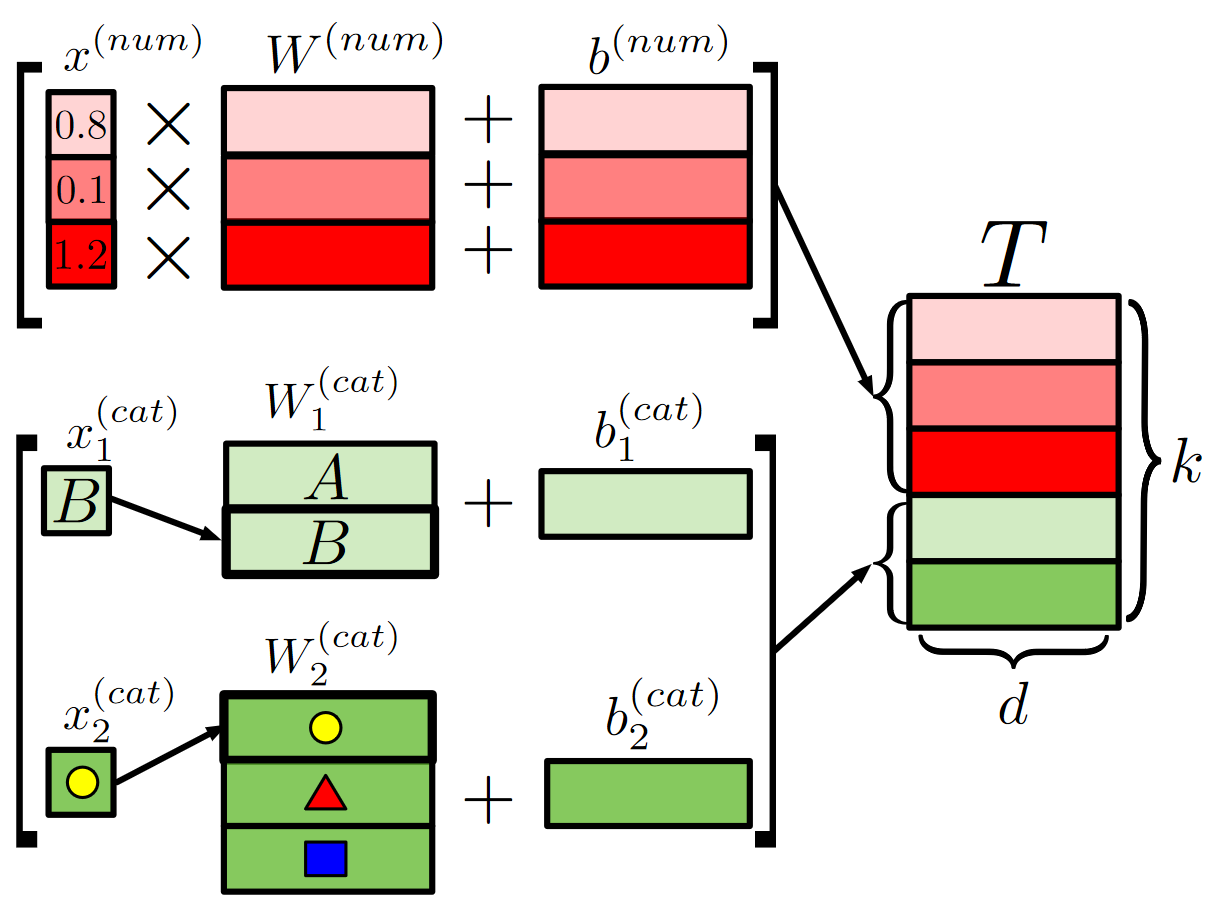
\includegraphics[width=0.5\textwidth]{images/ft.png}
	\caption[Feature Tokenization]{Feature Tokenization \cite[Figure 2a, p.4]{gorishniy2021RevisitingDeepLearning}}
	\label{fig:ft}
\end{figure}

To revert the synthetic data that the diffusion model produces to the original data format, the numerical and categorical columns need to be handled differently.
The corresponding embedding weights divide the numerical output element-wise, and the average value is computed as the final output \cite{zheng2022DiffusionModelsMissing}.
This transforms output having the same dimensionality as the embedding ($d$) back into a single value \cite{zheng2022DiffusionModelsMissing}.
For categorical output, the closest categorical embedding is determined by computing the Euclidean distance between the produced output and every categorical embedding \cite{zheng2022DiffusionModelsMissing}.

In the original work of \cite{gorishniy2021RevisitingDeepLearning}, the feature tokenizer is directly applied in front of a transformer model, allowing the gradients to flow through the embedding and linear layers during training.
This enables the model to learn a meaningful embedding.
In the adaptation of \cite{zheng2023DiffusionModelsMissing} and in this thesis, the weights of the layers are frozen.
Hence, learning is not possible, and the embedding is static.
The reason for this in this thesis have been because of the overall software architecture.
The data transformation and the actual model training are fully separated,
resulting in gradients that do not flow back to the feature tokenizer to update any weights of the embeddings.
To achieve the update of weights, the tokenizer would need to be fully integrated into the diffusion model architecture, which in turn could have negatively affected the overall maintainability, compatibility, and performance (see R2-R4, \autoref{ch:requirements}) of the software.

\subsection{Changes to the existing software}
\label{ch:methods-changes}
The changes made to the existing software (\autoref{ch:conceptualDesign-existingCodeBase}) are various and include multiple major changes as well as a lot of small changes.
Below, the major changes to the individual scripts are listed.
An additional visualization of the process of the scripts can be found in Appendix \ref{A:activity_diagrams}

\begin{description}
	\item[train.py:]
		Before the dataset is preprocessed and transferred into a dataset class, the \textit{TabularDataController} handles the tabular processing mechanisms.
		For this, a \textit{TabularDataController} is instantiated at the beginning and either loads a previously fit \textit{TabularProcesser} instance or fits and saves the \textit{TabularProcesser} on the training data.
		It receives context information on which tabular processing mechanisms and which properties the dataset has through the configuration file and handles the
		instantiation, fitting, and transformation of the raw data.
		Despite the addition of the \textit{TabularDataController}, the actual training remained untouched.
		Hence, introducing a \textit{TabularProcesser} only changes the data format (and maintains the segmented data structure) the diffusion model will receive and does not change the actual training loop.

	\item[sample.py:]
		A TabularDataController is instantiated at the beginning and loads a previously fit \textit{TabularProcesser} instance.
		If there is no previous \textit{TabularProcesser} instance to be loaded, it will call the fit function again.
		After the sampling is finished, the \textit{TabularProcesser}'s inverse transform function is called to bring the synthetic data into the original data format.

	\item[eval\_similarity.py:]
		This script does not replace the previous evaluation script.
		Instead, it is called after the original evaluation script (see \textit{pipeline.py}).
		First, three \textit{TabularDataController} instances are created, one for each train-, validation- and test data split.
		With the \textit{TabularDataController} instances, \gls{pd} \cite{mckinney-proc-scipy-2010} data frames are created, which are required for the TabSynDex similarity score.
		After the TabSynDex score is calculated, visualizations are created, if set by the user.

	\item[pipeline\_*.py:]
		The basic pipeline hardly changed.
		The only major change is that the similarity score evaluation is performed after the default evaluation using machine learning efficacy.
		In this evaluation, the TabSynDex metric is calculated as well as (if set by the user) visualization are created.

	\item[tune\_*.py:]
		Inside the tuning script, the objective function changed.
		If set by the user, the objective function will be based on the TabSynDex similarity score instead of the machine learning efficacy.
		To reduce processing time, visualizations inside the similarity evaluation part will, by default, only be created after the hyperparameters have been optimized and the eval\_seeds script will be executed.

	\item[eval\_seeds.py:]
		The basic eval\_seeds script did not change a lot.
		Again, the TabSynDex metric will be called after the default machine learning efficacy.
\end{description}

In order to easily change the \textit{TabularProcesser} type that should be executed in an experiment, the experiment configuration displayed as \autoref{lst:configuration} was extended.
The additional configuration section \textit{tabular\_processor} has been added, containing a \textit{type} key.
The \textit{type} key can be either set to "identity", "ft" or "bgm" to indicate, which \textit{TabularProcesser} type should be used.

\section{Experimental Setup}
\label{ch:methods-experimentalSetup}

\subsection{Experiments}
\label{ch:Experiments}

To systematically analyze the performance of the different tabular processing mechanisms, the following baseline experiments have been performed, creating a set of baseline models:

\begin{description}
	\item[Baseline-Real:] Comparison of the real training data with the real test data.
		The similarity evaluation is expected to be very high since the data is from the same joint distribution.
		The computed machine learning efficacy score can be seen as an objective value that should be reached.
		The closer the synthetic data based machine learning efficacy results are to this target, the better the synthetic data.
	\item[Baseline-TabDDPM:] Reproduction of the TabDDPM results of the authors \cite{kotelnikov2022TabDDPMModellingTabular} but with the extend evaluation explained in \autoref{ch:conceptualDesign-Evaluation} (Machine learning efficacy + TabSynDex + Visualizations).
	\item[Baseline-TVAE:] Like Baseline-TabDDPM but for TVAE.
	\item[Baseline-CTABGAN:] Like Baseline-TabDDPM but for CTABGAN.
	\item[Baseline-CTABGAN+:] Like Baseline-TabDDPM but for CTABGAN+.
	\item[Baseline-SMOTE:] Like Baseline-TabDDPM but for SMOTE.
\end{description}

\noindent For each implemented Tabular Processing mechanism, the following three experiments should be performed:

\begin{description}
	\item[Experiment 1:] Tabular Processing combined with TabDDPM with additional similarity evaluation. Hyperparameters tuned like in the original experiment (tuned after CatBoost-machine learning efficacy score).
	\item[Experiment 2:] Like Experiment 1, but hyperparameters are optimized towards the TabSynDex similarity score instead of the machine learning efficacy score.
	\item[Experiment 3:] Like Experiment 2, but the preprocessing strategy, that normalizes numerical data after the tabular processing transformation is replaced from a quantile transform function to a min-max transformation or is completely removed.
\end{description}

\noindent Depending on the results of the first experiments, subsequent experiments may only be performed on a subset of promising Tabular processing mechanisms.
To not get confused with the different model versions, the models are named after the following principal:
\begin{quote}
Modelname[-TabularProcessor]$^{tuning}_{preprocessing}$
\end{quote}
The Modelname is followed by an optional tabular processing mechanism.
The tuning strategy ("ml" for "machine learning efficacy score" or "s" for "TabSynDex similarity score") is indicated via a superscript (Experiment 2).
The preprocessing strategy ("q" for "quantile transform" or "m" for "min-max", or "n" for "none"/"no transformation") is indicated via a subscript (Experiment 3).

The min-max strategy was chosen as a commonly used linear transformation counterpart to the non-linear quantile transformation.
Since some tabular processing strategies already normalize or standardize the data, additional quantile or min-max transformations may not be required, 
which is why experiment 3 will also investigate the effect of applying no transformation after the tabular processor.

\subsection{Execution Environment}
\label{ch:environment}

The code was developed in python version 3.9.7 and made use of several libraries.
Most important libraries include (for a full list, please see the \textit{environment.yml} file in the source code):
\begin{itemize}
	\item azure-core, azureml-core: For running the code in the Microsoft Azure cloud \cite{microsoft2023CloudComputingServices}.
	\item catboost (1.0.3): contains the CatBoost model for the machine learning efficacy.
	\item pytorch (1.10.1): neural network framework.
	\item table\_evaluator (1.4.2): used to produce visualizations.
	\item numpy (1.21.4): allows efficient array computation.
	\item optuna (2.10.1): used for hyperparameter tuning.
	\item pandas (1.5.2): allows fast computations with dataframes of tabular data.
	\item scikit-learn (1.0.2): includes several utility functions for machine learning, \eg metrics such as accuracy or F1-score.
	\item TabSynDex \cite{chundawat2022UniversalMetricRobusta}: TabSynDex metric source code.
\end{itemize}

The training was performed using Microsoft Azure Machine Learning Studio.
Each experiment was executed on a STANDARD\_NC6 compute cluster running on Linux distribution, consisting of six virtual \glspl{cpu} (Intel Xeon E5-2690v3) with 56 GB Memory, 340 GB (SSD) Storage and the computing of one-half \gls{gpu} (Tesla K80) with 12 GB \gls{gpu} memory \cite{vikancha-msft2022NCseriesAzureVirtual}.
All experiments could also be performed locally on a Windows machine using a \gls{cpu}.
Local experiments with a \gls{gpu} should be possible but have not been tested.

\subsection{Hyperparameters}
The hyperparameter search space for the various models was not changed and is equal to the experiments in \cite{kotelnikov2022TabDDPMModellingTabular}.
The search space for the different models is listed in \Autoref{tab:catboost_tune,tab:diff_tune,tab:tvae_tune,tab:ctabgan_tune}. 
\begin{table}[h]
	\centering
	\begin{tabular}{lr}
		\toprule
		Parameter                 & Distribution        \\
		\midrule
		Max depth                 & UniformInt[3, 10]   \\
		Learning rate             & LogUniform[1e-5, 1] \\
		Bagging temperature       & Uniform[0,1]        \\
		L2 leaf reg               & LogUniform[1,10]    \\
		Leaf estimation iteration & UniformInt[1,10]    \\
		\midrule
		Number of tuning trials   & 100                 \\
		\bottomrule
	\end{tabular}
	\caption[CatBoost Hyperparameter Search Space]{CatBoost evaluation model hyperparameter tuning search space (proposed by \cite{gorishniy2021RevisitingDeepLearning})}
	\label{tab:catboost_tune}
\end{table}

\begin{table}[h]
	\centering
	\begin{tabular}{lr}
		\toprule
		Parameter               & Distribution                       \\
		\midrule
		Learning Rate           & LogUniform[1e-5,3e-3]              \\
		Batch Size              & Cat\{256,4096\}                    \\
		Diffusion timesteps     & Cat\{100,1000\}                    \\
		Training iterations     & Cat\{5000,10000,20000\}            \\
		\# MLP layers           & Int\{2,4,6,8\}                     \\
		MLP layer width         & Int\{128,256,512,1024\}            \\
		Proportion of samples   & Float\{0.25, 0.5, 1, 2\}           \\
		\midrule
		Train size              & \#entries in training dataset      \\
		\# Samples              & Proportion of samples * Train size \\
		Dropout                 & 0.0                                \\
		Scheduler               & cosine                             \\
		Gaussian diffusion loss & mse                                \\
		\midrule
		Number of tuning trials & 100                                \\
		\bottomrule
	\end{tabular}
	\caption[TabDDPM Hyperparameter Search Space]{TabDDPM model hyperparameter tuning search space}
	\label{tab:diff_tune}
\end{table}



\begin{table}[h]
	\centering
	\begin{tabular}{lr}
		\toprule
		Parameter               & Distribution                     \\
		\midrule
		\# classif. layers      & UniformInt[1,6]                  \\
		Classif. layer size     & Int\{62, 128, 256, 512\}         \\
		Training iterations    & Cat\{5000, 20000, 30000\}        \\
		Batch size              & Cat\{456,4096\}                  \\
		Embedding dim.          & Int\{16,32,64,128,256,512,1024\} \\
		Loss factor             & LogUniform[0.01, 10]             \\
		Proportion of samples   & Float\{0.25, 0.5, 1, 2, 4, 8\}   \\
		\midrule
		Number of tuning trials & 100                              \\
		\bottomrule
	\end{tabular}
	\caption[TVAE Hyperparameter Search Space]{TVAE model hyperparameter tuning search space}
	\label{tab:tvae_tune}

\end{table}

\begin{table}[h]
	\centering
	\begin{tabular}{lr}
		\toprule
		Parameter               & Distribution                   \\
		\midrule
		\# classif. layers      & UniformInt[1,4]                \\
		Classif. layer size     & Int\{62, 128, 256\}            \\
		Training iterations    & Cat\{1000, 5000, 7500\}        \\
		Batch size              & Int\{512,1024,2048\}           \\
		random dim.             & Int\{16,32,64,128\}            \\
		\# Channels             & Int\{16, 32, 64\}              \\
		Proportion of samples   & Float\{0.25, 0.5, 1, 2, 4, 8\} \\
		\midrule
		Number of tuning trials & 30                             \\
		\bottomrule
		\multicolumn{2}{c}{}\\[-0.2em] % Testen
	\end{tabular}
	\caption[CTABGAN(+) Hyperparameter Search Space]{CTABGAN/CTABGAN+ model hyperparameter tuning search space. Training iterations and the number of tuning trails were reduced compared to the original \cite{kotelnikov2022TabDDPMModellingTabular}, to reduce computation time.}
	\label{tab:ctabgan_tune}
\end{table}

\section{Dataset}
\label{ch:methods-datasets}

The dataset that was used for the experiments was the \textit{Adult} dataset, also known as "Census Income" from the UCI Machine Learning repository \cite{Dua:2019}.
The dataset was constructed through an extraction from a 1994 census database \cite{kohavi1996ScalingAccuracyNaiveBayes}.
Overall, the dataset has 15 columns, of which nine are categorical and six are numerical.
In total, the dataset consists of 48842 rows.

The numerical columns are: \textit{age}, \textit{fnlwgt}\footnote{short for "final weight", a sampling weight}, \textit{education-num}, \textit{capital-gain}, \textit{capital-loss} and \textit{hours-per-week}

And the categorical columns are: \textit{workclass}, \textit{education}, \textit{marital-status}, \textit{occupation}, \textit{relationship}, \textit{race}, \textit{sex}, \textit{native-country}, and \textit{income} (target column)

The dataset was created for binary classification, where the model should predict the column value of the income column (either \textit{>50K} or \textit{<=50K}).

\autoref{tab:adult} shows five entries of the dataset:


% \begin{table}[h]
% 	\centering
% 	\resizebox{\columnwidth}{!}{
% 		\begin{tabular}{|c|c|c|c|c|c|c|c|c|c|c|c|c|c|c|}
% 			\toprule
% 			\textbf{age} & \textbf{workclass} & \textbf{fnlwgt} & \textbf{education} & \textbf{education-num} & \textbf{marital-status} & \textbf{occupation} & \textbf{relationship} & \textbf{race} & \textbf{sex} & \textbf{capital-gain} & \textbf{capital-loss} & \textbf{hours-per-week} & \textbf{native-country} & \textbf{income} \\
% 			\midrule
% 			39.0         & State-gov          & 77516.0         & Bachelors          & 13.0                   & Never-married           & Adm-clerical        & Not-in-family         & White         & Male         & 2174.0                & 0.0                   & 40.0                    & United-States           & $\leq$50K       \\
% 			50.0         & Self-emp-not-inc   & 83311.0         & Bachelors          & 13.0                   & Married-civ-spouse      & Exec-managerial     & Husband               & White         & Male         & 0.0                   & 0.0                   & 13.0                    & United-States           & $\leq$50K       \\
% 			38.0         & Private            & 215646.0        & HS-grad            & 9.0                    & Divorced                & Handlers-cleaners   & Not-in-family         & White         & Male         & 0.0                   & 0.0                   & 40.0                    & United-States           & $\leq$50K       \\
% 			53.0         & Private            & 234721.0        & 11th               & 7.0                    & Married-civ-spouse      & Handlers-cleaners   & Husband               & Black         & Male         & 0.0                   & 0.0                   & 40.0                    & United-States           & $\leq$50K       \\
% 			28.0         & Private            & 338409.0        & Bachelors          & 13.0                   & Married-civ-spouse      & Prof-specialty      & Wife                  & Black         & Female       & 0.0                   & 0.0                   & 40.0                    & Cuba                    & $\leq$50K       \\
% 			\bottomrule
% 		\end{tabular}
% 	}
% 	\caption[Example Adult Dataset]{Adult income dataset with five exemplary entries}
% 	\label{tab:adult}
% \end{table}



\begin{table}[h]
	\centering
    \begin{subtable}{\textwidth}
        \centering
        \resizebox{\columnwidth}{!}{
            \begin{tabular}{|c|c|c|c|c|c|c|c|}
                \toprule
                \textbf{age} & \textbf{workclass} & \textbf{fnlwgt} & \textbf{education} & \textbf{education-num} & \textbf{marital-status} & \textbf{occupation} & \textbf{relationship} \\
                \midrule
                39.0         & State-gov          & 77516.0         & Bachelors          & 13.0                   & Never-married           & Adm-clerical        & Not-in-family         \\
                50.0         & Self-emp-not-inc   & 83311.0         & Bachelors          & 13.0                   & Married-civ-spouse      & Exec-managerial     & Husband               \\
                38.0         & Private            & 215646.0        & HS-grad            & 9.0                    & Divorced                & Handlers-cleaners   & Not-in-family         \\
                53.0         & Private            & 234721.0        & 11th               & 7.0                    & Married-civ-spouse      & Handlers-cleaners   & Husband               \\
                28.0         & Private            & 338409.0        & Bachelors          & 13.0                   & Married-civ-spouse      & Prof-specialty      & Wife                  \\
                \bottomrule
            \end{tabular}
        }
        \caption{First eight columns of Adult income dataset}
        \label{subtab:adult1}
    \end{subtable}
    \par\bigskip % add some space between the two tables
    \begin{subtable}{\textwidth}
        \centering
        \resizebox{\columnwidth}{!}{
            \begin{tabular}{|c|c|c|c|c|c|c|}
                \toprule
                \textbf{race} & \textbf{sex} & \textbf{capital-gain} & \textbf{capital-loss} & \textbf{hours-per-week} & \textbf{native-country} & \textbf{income} \\
                \midrule
                White         & Male         & 2174.0                & 0.0                   & 40.0                    & United-States           & $\leq$50K       \\
                White         & Male         & 0.0                   & 0.0                   & 13.0                    & United-States           & $\leq$50K       \\
                White         & Male         & 0.0                   & 0.0                   & 40.0                    & United-States           & $\leq$50K       \\
                Black         & Male         & 0.0                   & 0.0                   & 40.0                    & United-States           & $\leq$50K       \\
                Black         & Female       & 0.0                   & 0.0                   & 40.0                    & Cuba                    & $\leq$50K       \\
                \bottomrule
            \end{tabular}
        }
        \caption{Second seven columns of Adult income dataset, including the dataset target column "income"}
        \label{subtab:adult2}
    \end{subtable}
	\caption[Example Adult Dataset]{Adult income dataset with five exemplary entries}
	\label{tab:adult}
\end{table}

